\documentclass[11pt, letterpaper]{memoir}
\usepackage{HomeworkStyle}
\geometry{margin=0.75in}

\begin{document}
	\begin{center}
		{\large	Quiz 14.3 -- The Arrhenius Equation}
	\end{center}
	{\large Name: \rule[-1mm]{4in}{.1pt} 
	
	\noindent
	
	\subsection*{Question 1}
	Name the two conditions required for a molecular encounter to lead to reaction
	
	\vspace{3em}
	\begin{minipage}{0.4\linewidth}
		\noindent \hspace{-2em} \includegraphics[width=1.1\linewidth]{Simple_Rx_Coordinate} 
	\end{minipage}\hspace{1em}
	\begin{minipage}{0.49\linewidth}
		\subsection*{Question 2}
		Give the name for each item labeled on the reaction coordinate diagram at left
		\begin{description}
			\item[A:] ~
			\item[B:] ~
			\item[C:] ~
			\item[D:] ~
			\item[E:] ~
		\end{description}
	\end{minipage}
	
	
	\noindent A reaction is carried out at two temperatures, with the rate constant carefully measured. Data are given below:
	
	\begin{minipage}{0.25\linewidth}
		\begin{tabular}{c|c}
			$T\left(^\circ C\right)$ & $k\left(M^{-1}s^{-1}\right)$ \\ \midrule
			$15.00$ & $1.6\times10^{-4}$ \\
			$42.00$ & $8.7\times10^{-4}$
		\end{tabular}
	\end{minipage}\hspace{1em}
	\begin{minipage}{0.74\linewidth}
		\subsection*{Question 3}
		Give the activation energy and frequency factor for this reaction
	\end{minipage}
	
	\vspace{12em}
	\subsection*{Question 4}
	What is the overall reaction order for the reaction from Question 3?
	
	\newpage
	\newgeometry{margin=1.25in}
	\pagestyle{empty}
	\addtocounter{page}{-1}
	\section*{\emph{Who Has Seen the Wind?}}
	\paragraph{By Christina Rossetti}~
	\begin{verse}
		Who has seen the wind?\\
		Neither I nor you:\\
		But when the leaves hang trembling,\\
		The wind is passing through.
		
		Who has seen the wind?\\
		Neither you nor I:\\
		But when the trees bow down their heads,\\
		The wind is passing by.
	\end{verse}
\end{document}
